\documentclass{article}
\usepackage[spanish]{babel}
\usepackage[numbers,sort&compress]{natbib}
\usepackage[T1]{fontenc}
\usepackage[ansinew]{inputenc}
\usepackage{graphicx}
\usepackage{url}
\usepackage[numbers,sort&compress]{natbib}

\title { Movimiento Browniano}
\author{Anahi Llano}

\begin{document}

\maketitle

\section{Introducci\'on}\label{intro}

El movimiento browniano es un movimiento que ocurre de manera aleatoria observable en particulas microscopicas que se encuentran en un medio fluido, como es el polen en una gota de agua. tal movimiento recibe su nombre en honor al biologo botanico Robert Brown, quien en 1827 observo como es que las particulas de polen se despazablan de manera aleatoria sin alguna razon. El movimiento aleatorio de estas part\'iculas se debe a que su superficie es bombardeada incesantemente por las mol\'eculas, es decir, los \'atomos del fluido sometidas a una agitaci\'on t\'ermica. \citet{baz}
A pesar de que fue Robert Brown el primero el observar este fenomeno, el primero en explicarlo fue Einstein en 1905.
cuando se realiza una simulacion del movimiento browniano este se representa en movimientos tratandose de una caminata, en donde la particula parte desde un origen y esta da "pasos" discretos (tiempo) de forma aleatoria, realizandose desde una dimension hasta las que podamos imaginar tratandose de un modelo matematico. \citep{Eli}. con estos estudios es posible predecir las tendencias del comportamiento de las particulas de acuerdo a las diferentes variables que sean tomadas en cuenta.

/section{objetivo}\label{objec}

observar  los efectos de la dimensi\'on en el tiempo de regreso al origen del movimiento Browniano para dimensiones 1 a 8 en incrementos lineales de uno, variando el n\'umero de pasos de la caminata como potencias de dos con exponente de 5 a 10 en incrementos lineales de uno, con 50 repeticiones del experimento para cada combinaci\'on


\section{Metodolog\'ia}\label{met}

Se utiilizo el paquete estadistico R en la vercion 4.0.2 para estudiar los efectos de la dimensi\'on en el tiempo de regreso al origen del movimiento Browniano.
La practica consistio en simular una caminata variando las dimensiones entre 1 y 8 y tambi\'en los pasos de la misma como potencias de dos con exponente de 5 a 10 en incrementos lineales de uno.  Se realizaron 50 repeticiones para cada caso, con estos datos se
calcul\'o la probabilidad de regreso para cada una de las 8 dimensiones, as\'i mismo, se observ\'o el efecto de la dimension en el tiempo de regreso del origen de la caminata sobre el comportamiento de la particula.

los resultados obtenidos fueron graficados por medio de diagrama de caja y bigotes, en el cual se observa el efecto de la dimesion en el tiempo de regreso al origen de la particula en la cual se representa tal movimiento.

\section{Resultados y Discusi\'on}\label{res}

Una vez ejecutada la simulacion por medio de R, se obtuvieron una matriz de datos correspondientes a los porcentajes de regreso al punto de origen para cada dimension asi como cada duracion de la caminata. En la tabla \ref{t1} se muestra el conjunto de datos con el cual se realizo el analisis de la presente.

\begin{table} 
\caption{una parte de los datos obtenidos por medio de R ; la salida completa se encuentra en el repositorio de la tarea1}
\label{t1}
\begin{center}
\begin{tabular}{rrr}
\texttt{pot} & \texttt{porc} & \texttt{dim} \\
5  &  96  &  1 \\
5  &  80  &  2 \\
5  &  32  &  3 \\
5  &  16  &  4 \\
5  &  8    &   5 \\
5  &  14  &   6 \\
5  &  4    &   7 \\
5  &  14  &   8 \\
$\vdots$ &   $\vdots$ &   $\vdots$ \\
10  &   70  &  2 \\
10  &  24   &  3 \\
10  &  14   &  4 \\
10  &   6    &  5 \\
10  &  14   &  6 \\
10  &  8     &  7 \\
10  &  8     &  8 \\
\end{tabular}
\end{center}
\end{table}

Una vez obtenida la matriz de datos se construyo el diagrama de caja/bigote para observar como es que se comporta una particula con movimiento browniano (figura \ref{fig:pr1sim.png}) en donde cada caja corresponde a una dimension donde se ven agrupados los porcentajes de regreso al punto de origen en los diferentes tiempos de la caminata.

\begin{figure}
  \begin{center}
    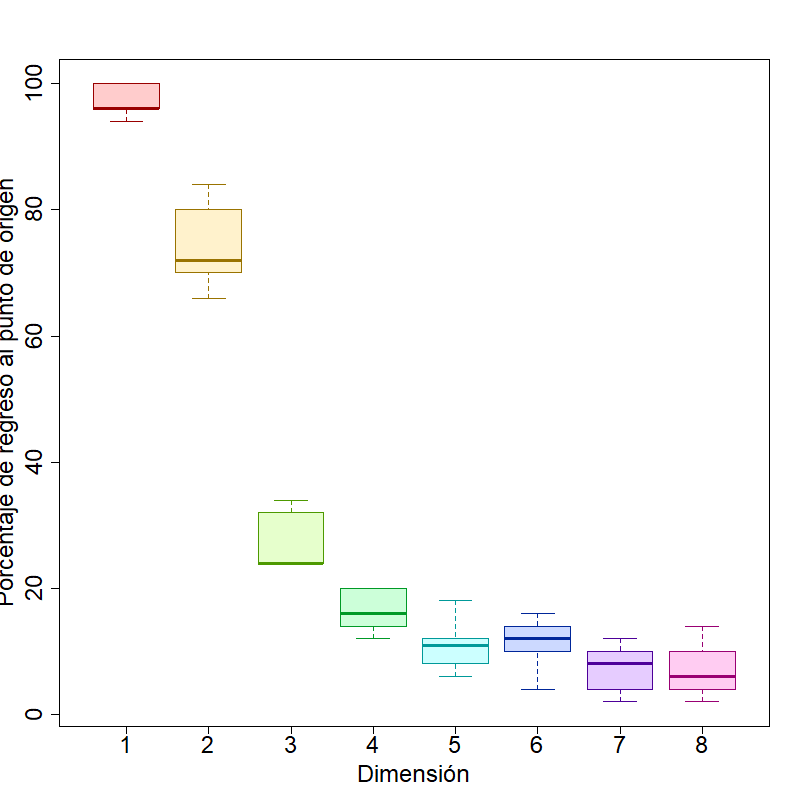
\includegraphics[width=10cm]{pr1sim.png}
  \end{center}
  \caption{porcentaje de regreso por dimensi\'on.}
  \label{fig:pr1sim.png}
\end{figure}

\section{conclusiones}\label{con}

Estubo interesante  en la seccion

\bibliographystyle{plainnat}
\bibliography{simu.bib}
\end{document}




